\documentclass{article}
\usepackage[spanish]{babel}
\usepackage[utf8]{inputenc}
\usepackage[top=20mm, bottom=20mm, left=15mm, right=15mm]{geometry}
\usepackage{amsmath}
\usepackage{graphicx}
\usepackage{float}
\usepackage{listings}
\usepackage{color}
\usepackage[all]{xy}
\definecolor{codeblue}{RGB}{0,128,255}
\definecolor{codegray}{rgb}{0.5,0.5,0.5}
\definecolor{codepurple}{rgb}{0.58,0,0.82}
\definecolor{pink}{RGB}{255,26,117}
\definecolor{backcolour}{rgb}{1,1,1}
    
\lstdefinestyle{mystyle}{
    backgroundcolor=\color{backcolour},
    commentstyle=\color{codeblue},
    keywordstyle=\color{pink},
    numberstyle=\tiny\color{codeblue},
    stringstyle=\color{codepurple},
    basicstyle=\footnotesize,
    breakatwhitespace=false,         
    breaklines=true,                 
    captionpos=b,                    
    keepspaces=true,                 
    numbers=left,                    
    numbersep=7pt,                  
    showspaces=false,                
    showstringspaces=false,
    showtabs=false,                  
    tabsize=2,
    frame=tb
}

\lstset{style=mystyle}

\title{
    Reconocimiento de letras manuscritas con redes neuronales artificiales\\ 
    \large Tercera y cuarta entrega}
\author{Edson Raul Cepeda Marquez \\ Sonia Alejandra Treviño Rivera}
\date{\today}

\begin{document}
\setlength{\parskip}{2mm}
\setlength{\parindent}{0pt}
\maketitle
\section{Resumen}\label{sec:Resumen}
Este proyecto esta alojado en un repositorio publico, todo código correspondiente fue escrito en ingles para asegurar la mayor accesibilidad. 
El proyecto consiste en una aplicación web que implementa una red neuronal artificial capaz 
de reconocer letras manuscritas. La aplicación web en cuestión está desarrollada con tres tecnologías 
que se conectan y permiten su uso:
\begin{enumerate}
    \item \textbf{Angular}: Un framework de código libre desarollado por Google que facilita el desarrollo de 
    aplicaciones web de una sola página (SPA: Single Page Applicaction). Tiene la ventaja de separar completamente el frontend y el backend lo que permite
    seguir facilmente el patrón de diseño MVC (Modelo-Vista-Controlador). 
    \item \textbf{Express}: Un framework de desarrollo web que utiliza el entorno de ejecución Node JS y facilita la creación de REST APIs.
    \item \textbf{Python}: Un lenguaje de programación interpretado orientado a objetos. Tiene la ventaja de ser simple, lo que permite escibir código legible.
    Tiene una amplia comunidad de desarrollo y una gran cantidad de librerias para todo tipo de tareas.
\end{enumerate}
En la figura \ref{flujo} se muestra un diagrama que representa el flujo de información entre las tres tecnologías. Se puede observar que la información fluye en ambas direcciones. 
\begin{figure}[H]
    \begin{displaymath}
        \xymatrix{*+<1cm>[F]{Angular} \ar[r] & *+<1cm>[F]{Express} \ar[l] \ar[r] & *+<1cm>[F]{Python} \ar[l]}
    \end{displaymath}
    \caption{Flujo de información de la aplicación.}
    \label{flujo} 
\end{figure}

La aplicación web además de contener este proyecto, tiene otras secciones asignadas para proyectos futuros. Para este proyecto la sección importante es ``Imchar''. 
Esta sección de la aplicación web contiene una cuadricula con la que se puede interactuar a traves del ratón. 
\begin{figure}[H]
    \centering
    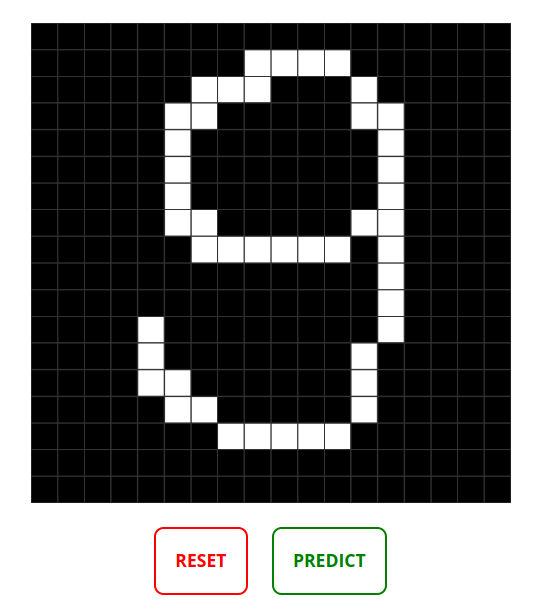
\includegraphics[width=40mm]{grid2.png}
    \caption{Cuadricula de la aplicación.}
    \label{grid}
\end{figure}
Esta es la puerta para el uso de la red neuronal artificial. 
En esta cuadricula es posible dibujar letras.
\\ Al dibujar una letra en la cuadricula y presionar el botón de ``Predeict'' la aplicación web realiza una petición al servidor de la REST API de express,
la cual recibe el estado de la cuadricula y sus dimensiones. \\
Posteriormente el servidor de express ejecuta un proceso asincrono de python el cual ejecuta un script que lleva a cabo una transformación de los datos enviados en la petición  \\
Por ultimo los datos transformados de la cuadricula son procesados por la red neuronal previamente entrenada, y devuelve una respuesta al frontend convertida en el caracter que la red neuronal predice (Figura \ref{response}).
\begin{figure}[H]
    \centering
    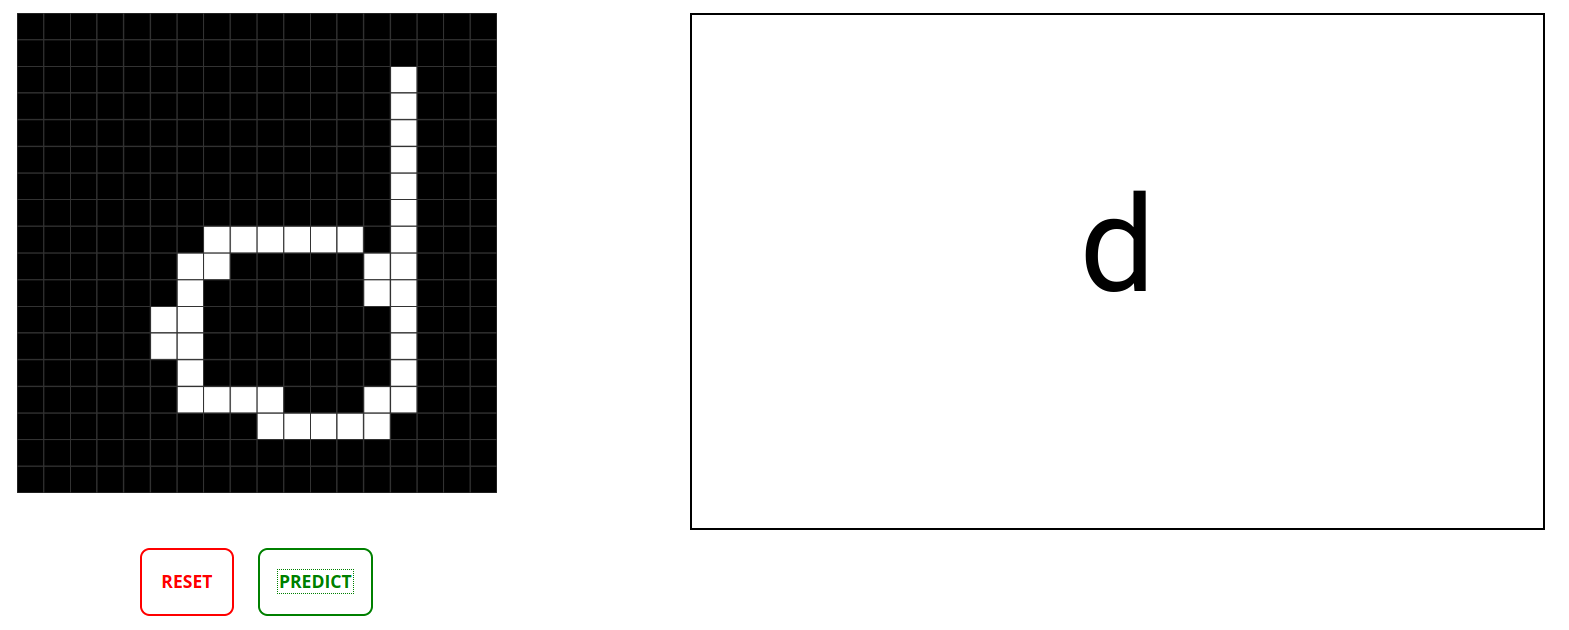
\includegraphics[width=180mm]{response.png}
    \caption{Respuesta de la red neuronal, también incluye el botón ``Reset'' para borrar la cuadricula.}
    \label{response}
\end{figure}
\textbf{Para el desarrollo de la red neuronal artificial no se utilizo ninguna librería, todo código correspondiente al algoritmo de aprendizaje fue escrito desde cero.} \\
Así mismo la red neuronal que procesa la información fue entrenada con un conjunto de datos creado desde cero, para esto se implemento una ruta oculta (figura \ref{trainer}) en la aplicación web en la que es posible utilizar la cuadricula para generar 
un conjunto de entranamiento.
\begin{figure}[H]
    \centering
    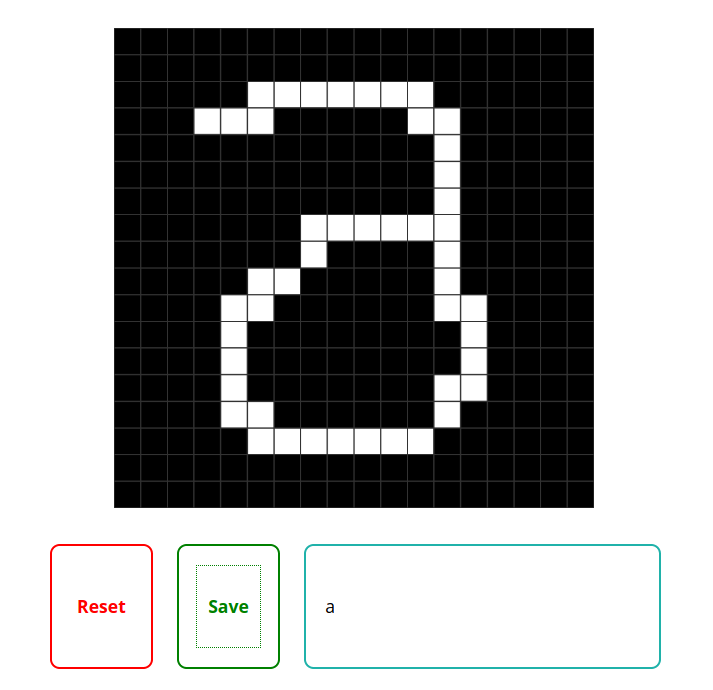
\includegraphics[width=60mm]{trainer.png}
    \caption{Ruta oculta para la generación de datos de entrenamiento}
    \label{trainer}
\end{figure}
Los resultados de entrenar la red neuronal con estos datos son que, para las 26 letras del abecedario en ingles por lo menos 21 son predichas correctamente. Las letras que presentan más problemas para ser predichas correctamente son aquellas que 
comparten cierta similaridad. La red neuronal fue entrenada multiples veces para poder llegar a una configuración de hiperparametros con un mejor rendimiento. 

\section{Introducción}\label{sec:Introduccion}
El problema que se intenta resolver al diseñar este sistema, es el de reconocer texto manuscrito para su digitalización. 
Se diseña una red neuronal convolucional que es entrenada con un conjunto de datos que contiene pequeñas imagenes de letras del abecedario en ingles. 
En la sección \ref{sec:Resumen} de este documento, se indica en que consiste el proyecto.  \\
La teoría necesaria para la realización de este proyecto se encuentra en la sección \ref{sec:Marco} \\
En la sección \ref{sec:Desarrollo} se revisa la implementación a detalle del sistema al igual que el diseño de la red neuronal. 
Por utlimo en la sección \ref{sec:Conclusion} se incluye una conclusión de lo que fue el proyecto incluyendo una introspección del equipo y trabajo a futuro. 
Todas la referencias utilizadas para este proyecto se incluyen en la sección de referencias.

\section{Marco teórico}\label{sec:Marco}
Una red neuronal artificial es un modelo matemático y un algoritmo de aprendizage automático inpirado en el funcionamiento de las neuronas biologicas que se encuentran en el cerebro.
El elemento básico de una red neuronal es la neurona. Una neurona se compone de cuatro partes fundamentales:
\begin{enumerate}
    \item \textbf{Dendrita}: Son ramificaciónes que conectan con el el cuerpo celular de una neurona, es la parte encargada de transportar los impulsos electricos.  
    \item \textbf{Cuerpo celular}: Es la parte de la neurona encargada de procesar la suma de los impulsos electricos recibidos de las dentritas. Posteriormente, se decide si disparara otra señal electrica de salida por el axon mediante un umbral.
    \item \textbf{Axon}: Son las ramificaciones finales de la neurona, transportan el impulso de salida de la neurona tras haber sido procesado en el cuerpo celular.
    \item \textbf{Sinapsis}: El punto de contacto entre el axon de una neurona y la dendrita de otra neurona. 
\end{enumerate} 
Es la organización de las neuronas y la fuerza de las sinapsis lo que establece la función principal de una neurona. En la figura \ref{neuron} se puede observar cada una de las partes de la neurona. 
\begin{figure}[H]
    \centering
    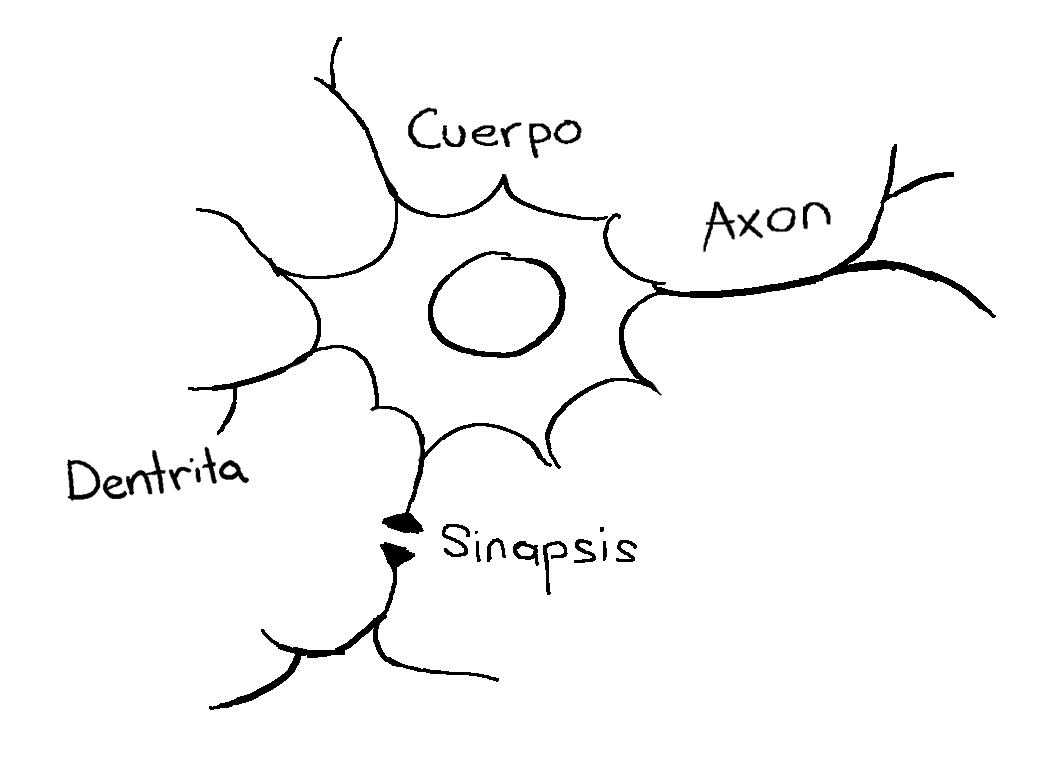
\includegraphics[width=130mm]{neuron.png}
    \caption{Neurona biologica}
    \label{neuron}
\end{figure}
Con esto es posible construir un modelo matemático de una neurona artificial (figura \ref{modelo}). En este modelo se tiene un escalar $p$ que corresponde a la señal del impulso electrico recibido de otras neuronas, $p$ es multiplicado por $w$ que corresponde a la fuerza de la sinapsis. 
Este producto $wp$ es enviado a una sumatoria y se incluye una entrada de sesgo $b$ con un valor de 1. La salida de la sumatoria $n$ va a una función de activación $f$ lo cual produce un escalar de salida $a$.
\begin{figure}[H]
    \centering
    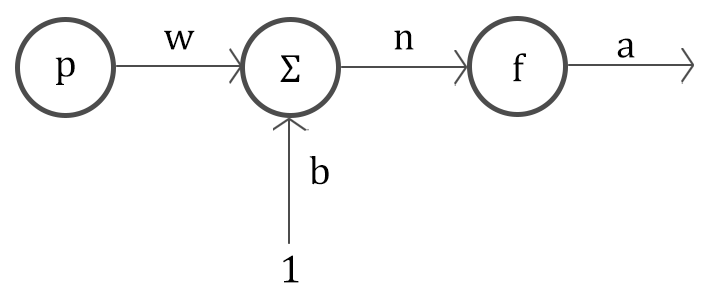
\includegraphics[width=85mm]{model.png}
    \caption{Modelo matemático de neurona artificial.}
    \label{modelo}
\end{figure}
De esta manera la salida de la neurona es calculada de la forma $a = f(wp + b)$. \\
La organización de multiples capas y multiples neuronas es lo que le da el poder a este algoritmo. A esto se le conoce como \textbf{red neuronal profunda}. 
Una red neuronal es también conocida como un aproximador de funciones universal, puesto es capaz de aproximar cualquier función teniendo la configuración adecuada.\\
El modelo matematico de una capa de una red neuronal profunda es, un vector \textbf{p} de tamaño $R$ como entrada,un determinado número de neuronas $S$, seguido de una matriz de pesos \textbf{W} con un tamaño $S\times$$R$ y un vector \textbf{b} de sesgo de tamaño $S\times1$. 
La operación \textbf{Wp + b} es enviada a una sumatoria que resulta en un vector de resultados \textbf{n} de tamaño $S\times1$ y que se dirige a una función de activación $f$ que da una vector \textbf{a} de tamaño $S\times1$ como salida. La salida de una capa es la entrada de la otra.
Para definir la arquitectura de una red neuronal se necesita definir una serie de parametros:
\begin{enumerate}
    \item Número de capas
    \item Número de neuronas por capa
    \item Tasa de aprendizage
    \item Funciones de activación de las neuronas
    \item Función de error de la red
\end{enumerate}
A estos se les conoce como \textbf{hiperparametros de la red}. Una red neuronal profunda (figura \ref{multi}) recibe su nombre del hecho que tiene una cantidad considerable de capas intermedias llamadas \textbf{capas ocultas}.
\begin{figure}[H]
    \centering
    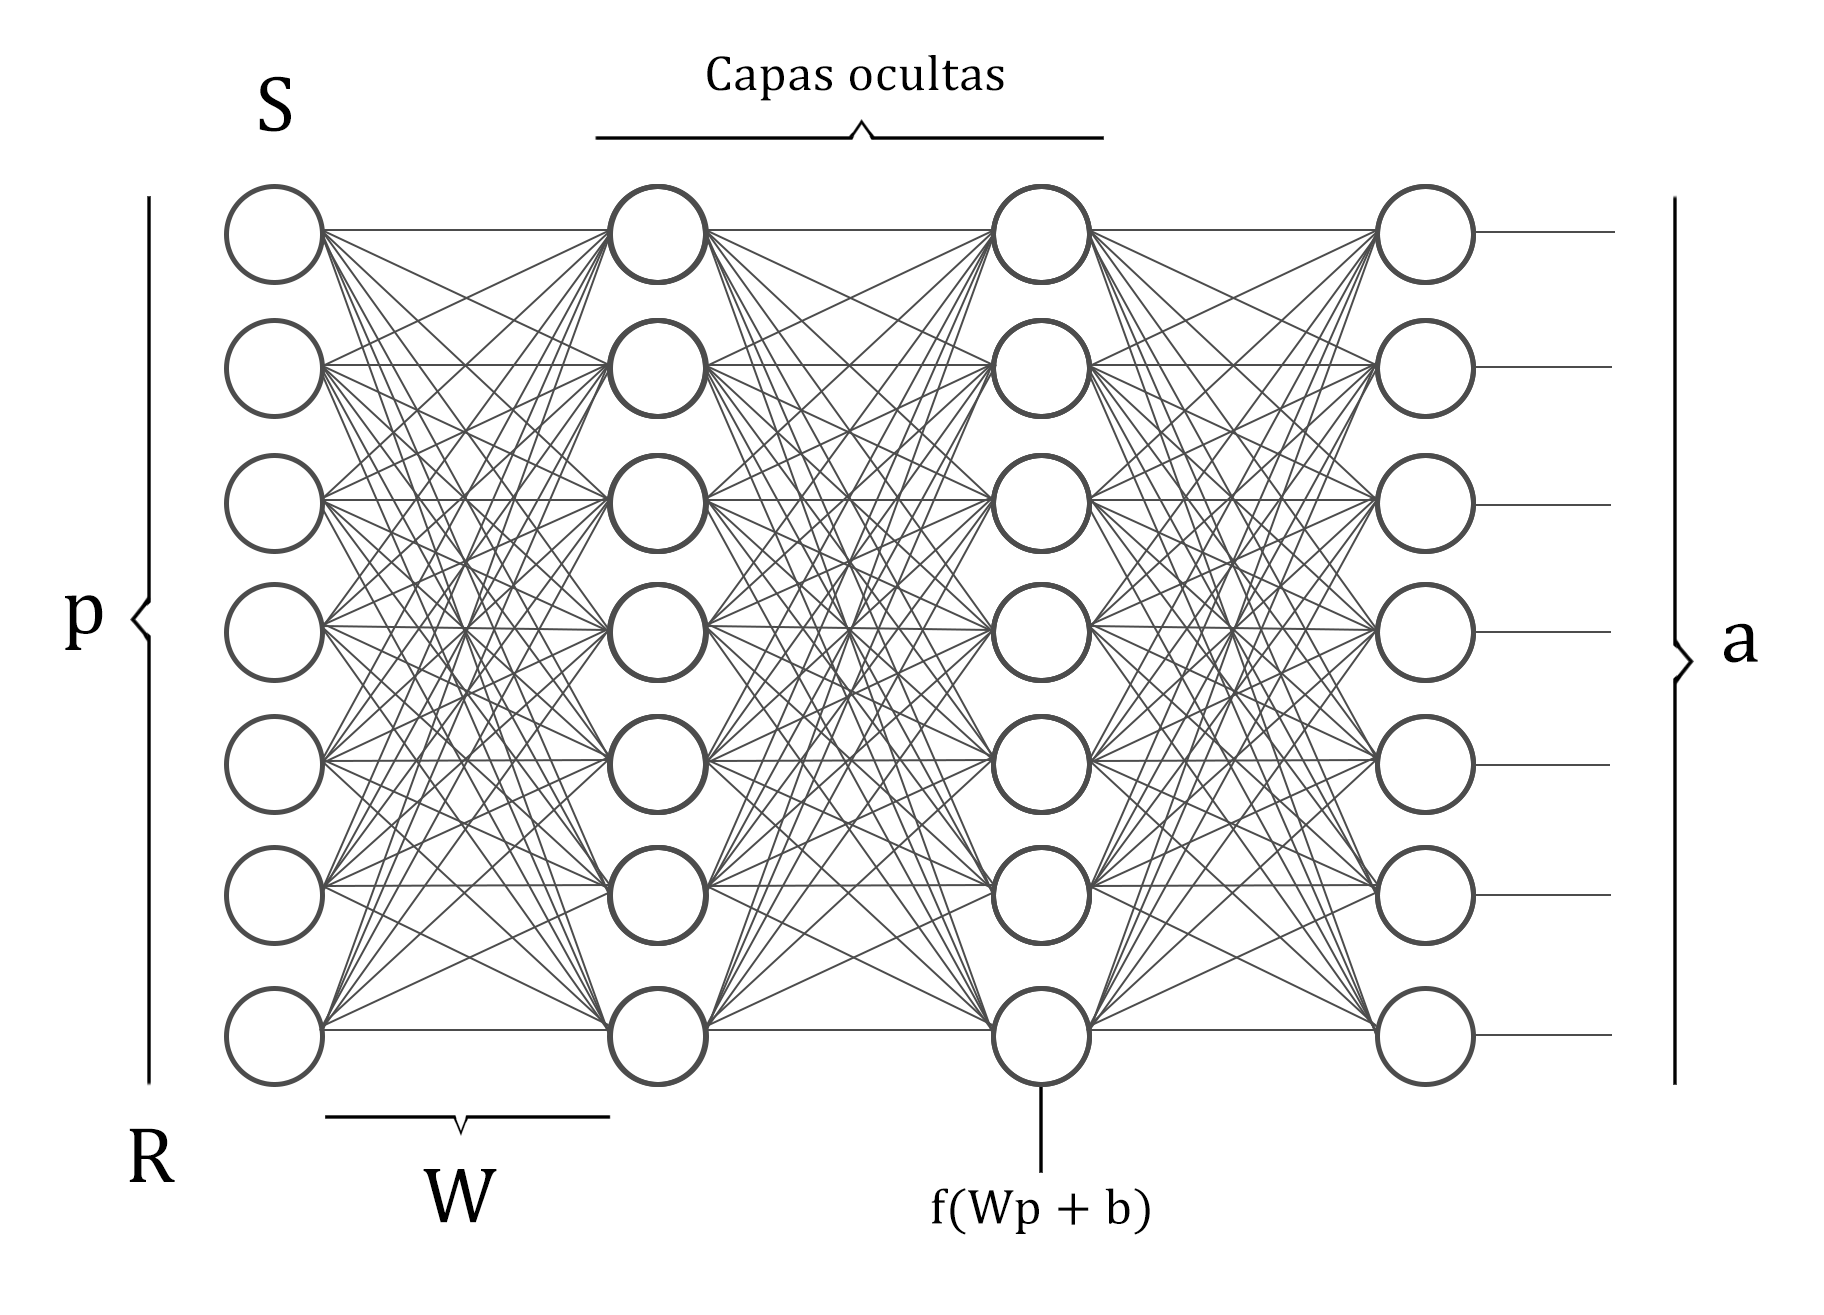
\includegraphics[width=100mm]{multi.png}
    \caption{Diagrama representativo de una red neuronal profunda}
    \label{multi}
\end{figure}
Al definir el número de neuronas de una capa también se tiene que escoger una función de activación adecuada.
Existen distintas funciones de activación que son comúnmente usadas en las redes neuronales. Las tres más comúnes son las siguientes:  \\
\textbf{Función sigmoidal o logistica}: Esta función se encuentra en el rango de 0 a 1. Es muy útil para modelos que requieren predecir una probabilidad. 
\begin{equation}
    f(x) = \frac{1}{1 + \exp^-x}
\end{equation}
\textbf{Función tangente hiperbolica}: Tambíen es una función logistica pero mejorada, el rango de esta función esta entre -1 a 1. Las ventajas de usar esta función es que penaliza fuertemente las entradas negativas. Es comúnmente usada para la clasificación de dos clases. 
\begin{equation}
    f(x) = \frac{1 - \exp^-2x}{1 + \exp^-2x}
\end{equation}
\textbf{ReLU (Unidad lineal rectificadora)}: Esta función es la más usada en las capas ocultas de las redes profundas puesto que evita el problema del desvanecimiento del gradiente que presentan las dos funciones anteriores. Esta función tiene un rango de 0 a infinito. 
Las entradas iguales o menores a cero se hacen cero, por lo que en algunos casos esto impide que se aprenda bien de los datos. Existen modificaciones de esta función que pretenden arreglar este problema como \textbf{Leaky ReLU} o \textbf{Randomized ReLU}. 
\begin{equation}
    f(x) = 
    \begin{cases}
        0, & x < 0 \\
        x, & x >= 0
    \end{cases}
\end{equation}
Las tres funciones anteriores son facílmente diferenciables lo que las hace adecuadas para el algoritmo de aprendizaje. El algoritmo más utilizado es el de propagación hacía atras o mejor conocido en ingles como \textbf{Backpropagation}. \\
Backpropagation es un algoritmo de aprendizaje que tiene como objetivo minimizar una función de error mediante el uso del \textbf{descenso del gradiente}. 
El entrenamiento de una red neuronal con este algoritmo consta de tres etapas:
\begin{enumerate}
    \item \textbf{Feedfoward}: Esta etapa consiste en propagar las entradas hacia delante en la red para obtener un resultado, este resultado se compara con el resultado esperado de la entrada y se calcula un error. 
    \item \textbf{Backpropagation}: Esta etapa consiste en calcular cuanto cambia el error si se ajustan cada uno de los pesos de la red neuronal. Se calcula una sensibilidad para los pesos derivando parcialmente la función de error respecto a cada peso. 
    \item \textbf{Actualización de pesos}: Usando las sensibilides calculadas en la etapa anterior se realiza una actualización en los valores de los pesos. 
\end{enumerate}
Este procedimiento es repetido multiples veces y con distintas entradas, estas son las \textbf{iteraciones} del entrenamiento. De esta manera la red es alimentada con suficientes ejemplos como para generalizar correctamente y reducir el error lo mejor posible.
Existen distintas architecturas que resuelven distintos tipos de problemas. Dos de las más comunes son:
\begin{enumerate}
    \item \textbf{Red neuronal convolucional}: es usada comúnmente para la clasificación de imagenes. Esta red neuronal consta de una serie de capas de extracción de caracteristicas que utiliza tecnicas de visión computacional. Las salidas de estas capas son conectadas con una serie de capas finales densas (totalmente conectadas) en las que se lleva a cabo el aprendizage.
    \item \textbf{Red neuronal recurrente}: es usada ampliamente en el campo de \textbf{procesamiento de lenguaje natural}, estas redes neuronal reciben su nombre debido a que existe una retroalimentación entre las capas.
\end{enumerate} 
Las redes neuronales como algoritmos de aprendizage automatico supervisado, realizan el proceso de aprendizage con conjuntos de datos previamente etiquetados. La calidad de este conjunto de datos refleja la calida de las predicciones de una red neuronal. \\
Otro de los factores que influyen en el rendimiento de la red neuronal, es la configuración de los hiperparametros. Existen problemas que requieren más o menos neuronas, otros que requieren más capas o menos capas. Es por esto que los hiperparametros de una red neuronal también pueden ser configurados automaticamente con el uso de otros algoritmos tales como \textbf{el algoritmo genetico}.

\section{Desarrollo}\label{sec:Desarrollo}
La técnica seleccionada es una \textbf{red neuronal convolucional}. Una red convolucional esta compuesta por una serie de capas con diferente organización, estas capas son:
\subsection{Capas de convoluciones}
Estas son las capas en la que se lleva a cabo la extracción de caracteristicas de una imagen. 
Las imagenes pueden ser representadas como matrices tridimensionales para imagenes en colores que corresponderian a cada uno de los canales (R: Rojo, G: Verde, B: Azul) o como matrices bidimensionales que representan imagenes en escala de grises (figura \ref{cat}). 
\begin{figure}[H]
    \centering
    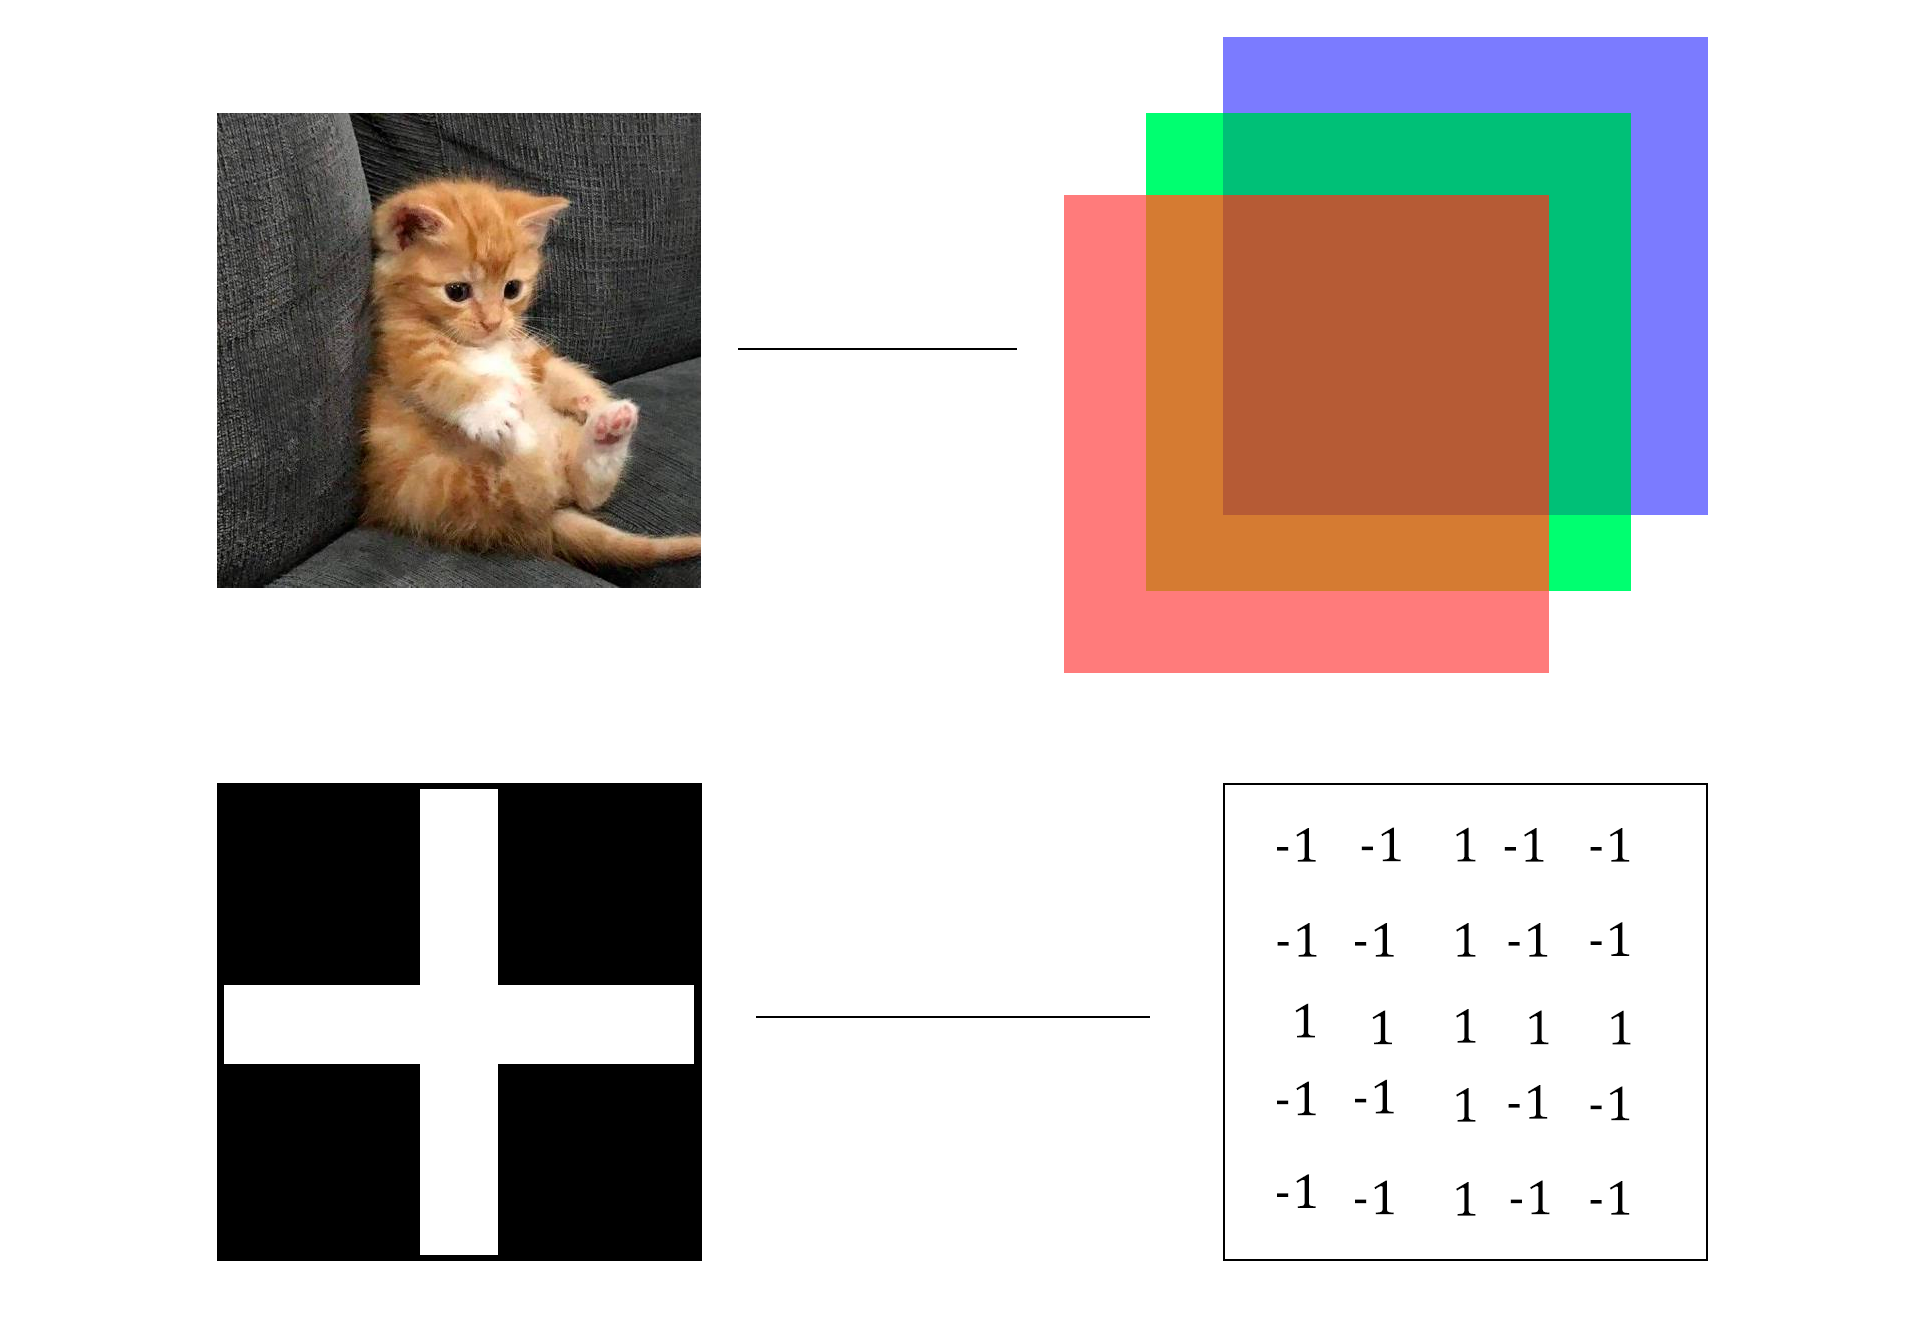
\includegraphics[width=115mm]{cat.png}
    \caption{Representación de imagenes en matrices}
    \label{cat}
\end{figure}
Una convolución se refiere al proceso de aplicar un filtro a una imagen, los filtros utilizados en estas capas son llamados \textbf{kernel}. Ejemplos comunes de kernels se pueden observar en la figura: 
\begin{figure}[H]
    \centering 
    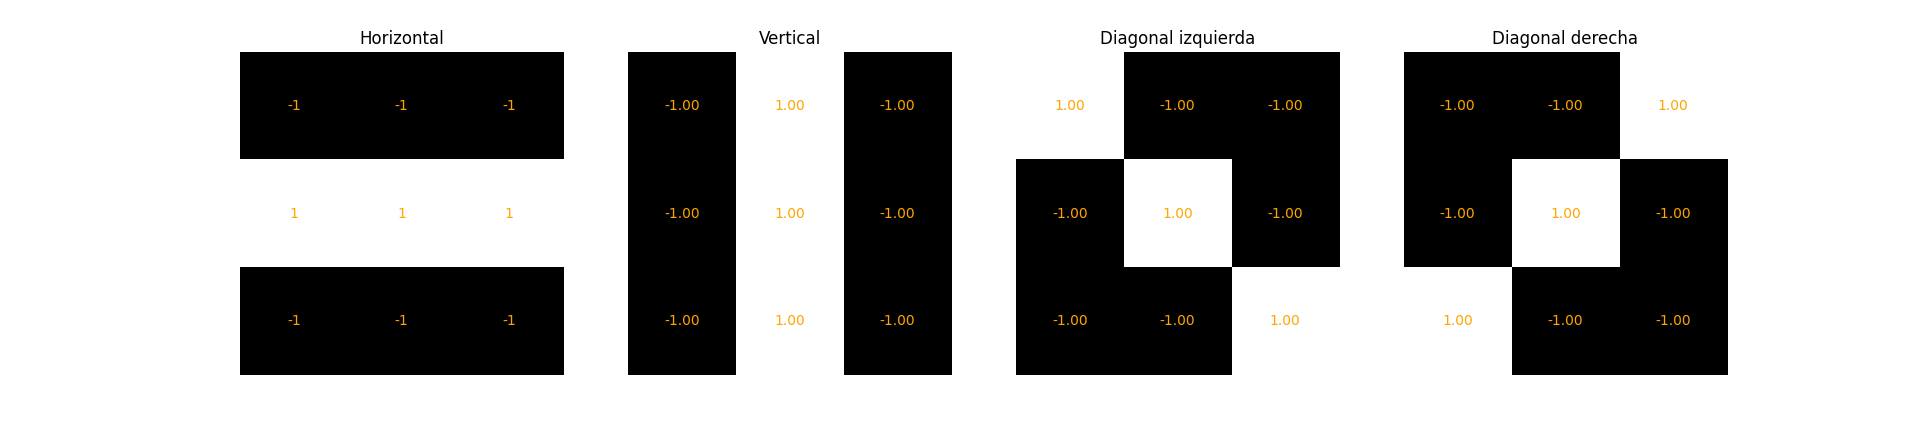
\includegraphics[width=170mm]{kernels.png}
    \caption{Representación de imagenes en matrices}
    \label{kernels}
\end{figure}
Estos kernels son pequeñas matrices que se desplazan sobre la imagen realizando un producto punto, el pixel central se cons de manera queerva y se origina una nueva imagen.A esta operación se le llama \textbf{correlación cruzada} De esta manera los elementos de la matriz que más encajan con la imagen se veran resaltados en la nueva imagen. Al realizar esta operación de convolución es común que se reduzca la dimensionalidad de la matriz original, por lo que se utiliza la técnica de \textbf{padding} que 
genera un borde de ceros para el pixel central del kernel encaje con el primer pixel de la imagen, de esta manera se conservan las dimensiones de la imagen original.
Para la implementación de esta técnica se creo una clase especializada que incluye la lógica del algoritmo de convolución. \\
Se crea un archivo en el que solo se declara las matrices de los kernels. Se incluye kernels para lineas verticales, lineas horizontales, lineas diagonales, difuminación, contornos, nitidez. \\
\begin{lstlisting}[language=python]
import numpy as np

horizontal_line = np.array([[-1,-1,-1],[1,1,1],[-1,-1,-1]])

vertical_line = np.array([[-1,1,-1],[-1,1,-1],[-1,1,-1]])

diagonal_left = np.array([[1,-1,-1],[-1,1,-1],[-1,-1,1]])

diagonal_right = np.array([[-1,-1,1],[-1,1,-1],[1,-1,-1]])

cross = np.array([[1,-1,1],[-1, 1,-1],[1,-1, 1]])

circular = np.array([[-1, 1, -1],[ 1,-1,  1],[-1, 1, -1]])

sharpening = np.array([[0,-1,0],[-1,5,-1],[0,-1,0]])

blur = np.array([[0.0625,0.125,0.0625],[0.125,0.25,0.125], [0.0625,0.125,0.0625]])

bottom_sobel = np.array([[-1,-2,-1],[0,0,0],[1,2,1]])

emboss = np.array([[-2,-1,0],[-1,1,1],[0,1,2]])

outline = np.array([[-1,-1,-1],[-1,8,-1],[-1,-1,-1]])

top_sobel = np.array([[1,2,1],[0,0,0],[-1,-2,-1]])

\end{lstlisting}

En un archivo separado se importan los kernels y se escribe la función que realiza la operación de correlación cruzada. Se empieza por definir los tamaños de las entradas
para poder recorrer ambas matrices, la de kernel con un tamaño $h\times$$w$ y la de entrada $H\times$$W$. La función puede ser ejecutada con un parametro opcional que es el del padding, en caso de que sea una valor verdadero 
se crea una matriz expandida con zeros en los borders. La matriz origina con un tamaño de $h\times$$w$ se ve expandida a una matriz de tamaño $(h+2)\times$$(w+2)$, esto debido a que se agrega una fila de ceros por encima, 
por debajo, por la izquieda y por la derecha. En caso de que el valor de padding sea falso, no se realiza la expansión y directamente se hacen las operaciones de correlación. De esta manera la nueva matriz que representa la imagen 
termina con un tamaño de $(H-h+expansion+1)\times$$(W-w+expansion+1)$. El valor de retorno de la función es la nueva matriz.  \\
\begin{lstlisting}[language=python]
import numpy as np 
import Kernels

def crossCorr2d(input, kernel,padding = False):
    h,w = kernel.shape #Dimensions of kernels
    H,W = input.shape #Dimensions of input matrix
    pad = 0
    expansion = 0
    if(padding):
        pad = 1
        expansion = pad * 2 #Two borders of zeros vertical and horizontal
        paddedInput = np.zeros((H+expansion, W+expansion))
        #Assigning old values in the center of the matrix with padding
        for i in range(input.shape[0]):
            for j in range(input.shape[1]):
                paddedInput[i+pad,j+pad] = input[i,j]
        #Replace the original input with the padded input matrix
        input = paddedInput
    output = np.zeros((H-h+expansion+1, W-w+expansion+1)) #Initializing new matrix
    for i in range(output.shape[0]):
        for j in range(output.shape[1]):
            output[i,j] = (input[i:i+h, j:j+w] * kernel).sum()/(h*w) #Asigning cross correlation operations
    return output
\end{lstlisting} 
Para comprobar el funcionamiento de la función, se exploran los resultados de aplicar seis kernels distintos a una misma imagen en escala de grises.  \\
Se hace uso de la librería matplotlib para la visualización de los resultdos. En la figura se puede observar como cambian los resultados con distitos kernels y cuales son las 
caracteristicas de la imagen que más se ven resaltadas con cada uno. 
\begin{figure}[H]
    \centering
    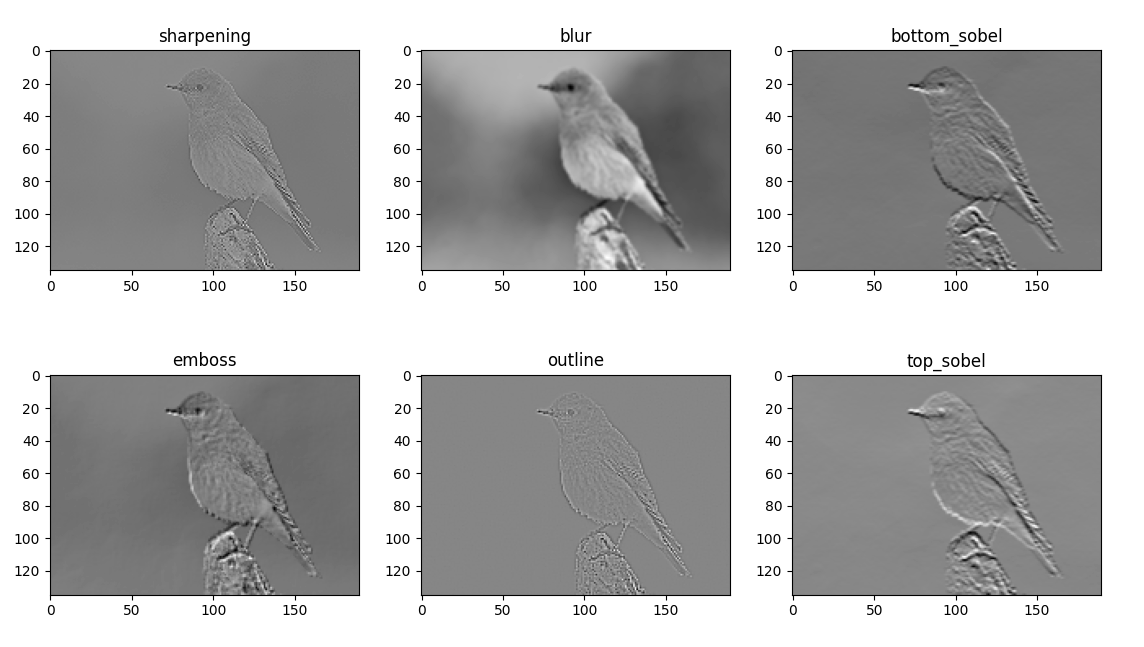
\includegraphics[width=180mm]{bird.png}
    \caption{Resultado de aplicar los kernels a la imagen}
    \label{bird}
\end{figure}
\subsection{Capas de pooling}
La operación de pooling realiza una reducción de dimensionalidad en una matriz, concretamente la técnica de \textbf{max pooling} funciona de la siguiente manera: \\
Se utiliza el concepto de una ventana con un tamaño determinado, que se desplaza en el interior de la matriz. La ventana se define por su tamaño y por los pasos que avanza.
Se toma el valor máximo de la ventana y se asigna a la nueva matriz reducida (figura \ref{pooling}).
\begin{figure}[H]
    \centering
    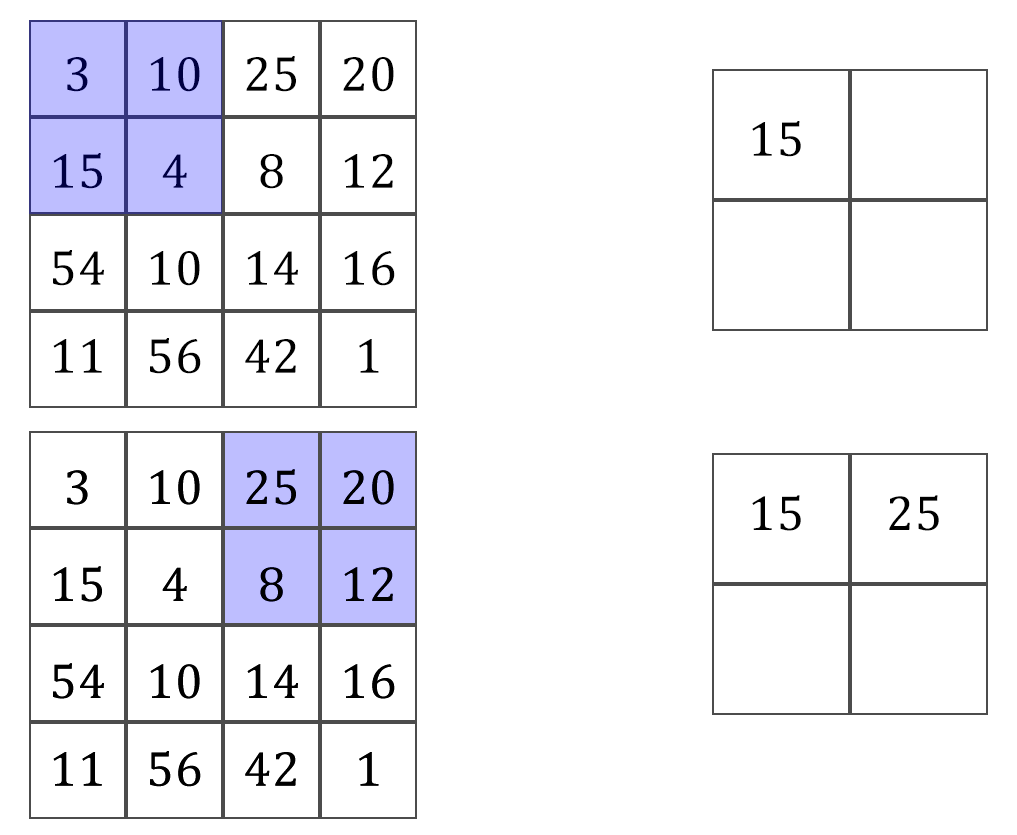
\includegraphics[width=80mm]{pooling.png}
    \caption{Representación de la operación de pooling}
    \label{pooling}
\end{figure} 
Se crea un archivo en donde se define la función de pooling, la función recibe como parametros una matriz, un entero que representa el tamaño de la ventana del pooling y un entero
que indica el desplazamiento de la ventana. 
\begin{lstlisting}[language=python]
import numpy as np 

def max_pooling(matrix, size, stride):
    h,w = matrix.shape #input matrix shape
    if h%2!=0: #If odd
        h=h+1
    if w%2!=0:
        w=w+1
    pooled_matrix = np.zeros((int(h/2),int(w/2))) #Final matrix size
    movey = 0
    for i in range(pooled_matrix.shape[0]):
        movex = 0
        for j in range(pooled_matrix.shape[1]):
            pooled_matrix[i,j] = (matrix[movey:movey+size,movex:movex+size]).max() #Check for maximum value
            movex += stride
            movey += stride #steps
    return pooled_matrix
\end{lstlisting}
\subsection{Capas ReLU}
Las capas de ReLU tienen como objetivo eliminar los números negativos y convertirlos en cero, de esta manera se dejan las caracteristias importantes de la matriz o imagen. Se crea un archivo y se define la función, de manera que
para cualquier elemento de una matriz que sea menor a cero este se convierte en cero. 
\begin{lstlisting}[language=python]
def RELU(matrix):
    new_matrix = matrix.copy()
    new_matrix[new_matrix < 0] = 0
    return new_matrix
\end{lstlisting}

\subsection{Red multicapa}
La parte final de una red convolucional es una red neuronal multicapa totalmente conectada. Se crea un archivo que contiene la clase ``NeuralNetwork''. 
La clase contiene una serie de metodos que implementa los algoritmos necesaarios para su funcionamiento, estos metodos son:

\textbf{Método \texttt{init}}: Inicializa la red neuronal, se calcula el número de capas de la red, y se asignan los demás parametros a variables de instancia.
Contiene dos parametros opcionales que son los pesos y los sesgos iniciales de la red, en caso de que la clase no sea instanciada con estos metodos se ejecutan los metodos \texttt{weightsInit} y \texttt{biasesInit}. 

\textbf{Método \texttt{weightsInit} y \texttt{biasesInit}}: Genera un serie de números aleatorios  con distribución normal que son guardados las matrices de pesos y sesgos, estas matrices son guardadas despues en una lista.

\textbf{Método \texttt{train}}:Este método contiene una serie de llamadas a otros metodos para realizar el entrenamiento, especificamente llama los metodos \texttt{forwardPass}, \texttt{backwardPass}.

\textbf{Método \texttt{forwardPass}}: Comprueba que función de activación fue asignada a cada capa y se realiza las operaciones correspondientes para generar un salida de la red. La salida de cada capa es guardada en una lista.

\textbf{Método \texttt{backwardPass}}: Este es el método más complejo de la red, en este se realiza el algoritmo de backpropagation. Primero calcula el error de la red, inicia una iteración para todas las capas y genera una matriz jacobiana que contiene
los resultados de aplicar la función derivada de cada capa a los ultimos resultados de la red. Cada matriz jacobiana es guardada en una lista. 
Dentro de la iteración se comprueba si se encuentra en la primera iteración, de ser así se calcula las sensibilidaes de los pesos de la ultima capa la cual esta directamente relacionada con el error. Estas sensibilidades son guardadas en una lista. 
En caso de no ser la primera iteración se utiliza la matriz jacobiana y las sensibilidades de las capas anteriores para calcular como se propaga el error.
Las ecuaciones correspondientes para el calculo de las sensibilides son las siguientes: 
Para el calculo de la salida de la red:
\begin{equation}
    a^0 = p
\end{equation}
Donde $a$ es el vector de resultados y $p$ es el vector de entradas. 
\begin{equation}
    a^{m+1} = f^{m+1}(W^{m+1}a^m + b^{m+1}) \hspace{1em} para \hspace{1em} m = 0, 1, ..., M -1
\end{equation}
Donde $a^{m+1}$ es el vector de resultado de la siguiente capa, $f^{m+1}$ es la función de activación de la siguiente capa, $W^{m+1}$ es la matriz de pesos que conecta con la siguiente capa,
$a^m$ es el vector de resultados de la capa anterior, $b^{m+1}$ es el vector de sesgos de la siguiente capa, $m$ corresponde a la capa acutal, y $M$ corresponde al número de capas totales.
De esta manera el vector de resultados final es:
\begin{equation}
    a = a^M
\end{equation}
Para el calculo de las sensibilidades se empieza por la capa final y termina en la capa inicial. De esta manera la sensibilidades de la capa final se calculan con:
\begin{equation}
    s^M  = -2F'^M(n^M)(t-a)
\end{equation}
Donde $s^M$ es la matriz de sensibilidades de la ultima capa $t$ es el vector de resultado esperado, $a$ es el vector actual de resultado y  $F'^M$ es la jacobiana definida a partir de las funciones de activación de la ultima capa que se expresa como: 
\begin{equation}
    F'^m(n^m) = \begin{bmatrix}
        f'^m(n_1^m) &  0 & \dots &  0     \\
        0 & f'^m(n_2^m) & \dots & 0 \\ 
        \vdots & \vdots & \hspace{1em} & \vdots \\
        0 & 0 & \dots & f'^m(n_{S^m}^m)
    \end{bmatrix} ,
\end{equation}
Para el calculo de las demás sensibilidades se usa:
\begin{equation}
    s^m = F'^m(n^m)(W^{m+1})^Ts^{m+1}, \hspace{1em} para \hspace{1em} m = M-1, ..., 2,1.
\end{equation}

\textbf{Método \texttt{weightsUpdate}}: En este método se realiza la actualización de los pesos, utilizando las sensibilides calculadas. Para esto se usa:
\begin{equation}
    W^m(k+1) = W^m(k) - \alpha s^m(a^{m-1})^T
\end{equation}
En donde $W^m(k+1)$ es la nueva matriz de pesos, $W^m(k)$ es la vieja matriz de pesos, $\alpha$ es la tasa de aprendizaje, $s^m$ es la matriz de sensibilidaes de la capa $m$,
$(a^{m-1})^T$ es el vector de resultados de la capa transpuesto. 

\textbf{Método \texttt{predict}}: Este método se utiliza para utilizar la red neuronal para procesar una entrada y obetener un respuesta. 

Los metodos \texttt{sigmoid}, \texttt{linear}, \texttt{RELU}, \texttt{softmax}, \texttt{tanh} se refieren a los métodos es los que se definen las distintas funciones de activación que pueden ser 
utilizadas en la red.

\textbf{Método \texttt{jacobian}}: Este método genera la matriz jacobiana tomando en cuenta la función de activación de la capa en la que se encuentra. 

El código correspondiente a la implementación desde cero de la red neuronal multicapa utilizando solamente numpy para el manejo de matrices es el siguiente:
\begin{lstlisting}[language=python]
import numpy as np

class NeuralNetwork():
    def __init__(self,neurons,activation,error_function,learning_rate, weights=None,biases=None):
        self.layers = len(neurons) - 1 #number of layers
        self.neurons = neurons #number of neurons per layer
        self.activation = activation
        self.error_function = error_function #Error function
        self.weights = weights
        self.biases = biases
        self.learning_rate = learning_rate
        self.jacobians_list = []
        if not self.weights:
            self.weightInit()
        if not self.biases:
            self.biasesInit()
    
    def weightInit(self):
        self.weights = []
        for i in range(self.layers):
            self.weights.append(np.random.normal(0, 0.01,size=(self.neurons[i+1],self.neurons[i])))
                
    def biasesInit(self):
        self.biases = []
        for i in range(self.layers):
                self.biases.append(np.random.normal(0,0.01,size=(self.neurons[i+1],1)))
            
    def train(self,inputs, target):
        self.outputs = [inputs]
        self.deltas = []
        self.forwardPass()
        self.backwardPass(target)
        self.weightsUpdate()
        
    def forwardPass(self):
        for i in range(self.layers):
            if self.activation[i] == "sigmoid":
                self.outputs.append(self.sigmoid(self.weights[i]*self.outputs[-1] + self.biases[i]))
            elif self.activation[i] == "linear":
                self.outputs.append(self.linear(self.weights[i]*self.outputs[-1] + self.biases[i]))
            elif self.activation[i] == "RELU":
                self.outputs.append(self.RELU(self.weights[i]*self.outputs[-1] + self.biases[i]))
            elif self.activation[i] == "softmax":
                self.outputs.append(self.softmax(self.weights[i]*self.outputs[-1] + self.biases[i]))
            elif self.activation[i] == "tanh":
                self.outputs.append(self.tanh(self.weights[i]*self.outputs[-1] + self.biases[i]))
            
    def backwardPass(self,targets):
        self.error = targets - self.outputs[-1]
        for i in range(self.layers):
            jacobian = self.jacobian(self.neurons[-1-i], self.activation[-1-i],self.outputs[-1-i])
            self.jacobians_list.append(jacobian)
            if i == 0:
                if self.error_function == "SE":
                    s = -2 * jacobian * (targets - self.outputs[-1-i])
                elif self.error_function == "MSE":
                    s = jacobian * (self.outputs[-1-i] - targets)
            else:
                rhs = self.weights[-i].T * self.deltas[-1]
                s = self.jacobians_list[-1] * rhs
            self.deltas.append(s)
    
    def weightsUpdate(self):
        for i in range(self.layers):
            self.weights[self.layers-1-i] -= self.learning_rate * self.deltas[i] * self.outputs[-2-i].T
            self.biases[self.layers-1-i] -= self.learning_rate * self.deltas[i]
    
    def predict(self,input):
        for i in range(self.layers):
            if self.activation[i] == "sigmoid":
                input = self.sigmoid(self.weights[i]*input + self.biases[i])
            elif self.activation[i] == "linear":
                input = self.linear(self.weights[i]*input + self.biases[i])
            elif self.activation[i] == "RELU":
                input = self.RELU(self.weights[i]*input + self.biases[i])
            elif self.activation[i] == "softmax":
                input = self.softmax(self.weights[i]*input + self.biases[i])
            elif self.activation[i] == "tanh":
                input = self.tanh(self.weights[i]*input + self.biases[i])
        return input
        
    def sigmoid(self,x,deriv = False):
        if deriv:
            return x * (1 - x)
        return 1/(1 + np.exp(-x))
    
    def linear(self,x, deriv = False):
        if deriv:
            return 1
        return x
    
    def RELU(self,x, deriv=False):
        if deriv:
            return np.where(x < 0, 0, 1)
        return np.where(x < 0, 0, x)
    
    def softmax(self,x, deriv = False):
        if deriv:
            return 1 / (1 + np.exp(-x))
        return np.log(1 + np.exp(x))
    
    def tanh(self,x,deriv=False):
        if deriv:
            return 1 - (x * x)
        return np.tanh(x)
        
    def jacobian(self,neurons,activation,x):
        result = np.zeros((neurons,neurons))
        x_counter = 0
        for i in range(neurons):
            for j in range(neurons):
                if i == j:
                    if activation == "sigmoid":
                        result[i,j] = self.sigmoid(x[x_counter],deriv=True)
                    elif activation == "linear":
                        result[i,j] = self.linear(x[x_counter],deriv=True)
                    elif activation == "RELU":
                        result[i,j] = self.RELU(x[x_counter],deriv=True)
                    elif activation == "softmax":
                        result[i,j] = self.softmax(x[x_counter],deriv=True)
                    elif activation == "tanh":
                        result[i,j] = self.tanh(x[x_counter],deriv=True)
                    x_counter += 1
        return result
\end{lstlisting}
La clas de la red neuronal recibe como parametros de instanciación, una lista que contiene el número de neuronas por capa, una lista que contiene las funciones de activación de las capas, un string que indica la función de error a utilizar y la tasa de aprendizaje. Los parametros para instanciar la red con pesos y sesgos iniciales son opcionales, y como se menciono anteriormente esos se inicializan automaticamente
con los métodos \texttt{weightsInit} y \texttt{biasesInit}.
Un ejemplo de instanciación de la clase de la red neuronal es el siguiente:
\begin{lstlisting}[language=python]
neurons = [2,4,4,2] #Number of neurons
activation = ["RELU","RELU","RELU","sigmoid"] #Activation functions
error = "SE" #Squared error function
lr = 0.1 #Learning rate
NN1 = NeuralNetwork(layers,neurons, activation,error,weights,biases, lr)
\end{lstlisting}
La red esta adaptada para manejar cualquier número de capas y neuronas. 
Este ejemplo de instanciación corresponde a la siguiente arquitectura mostrada en la figura \ref{inst}:
\begin{figure}[H]
    \centering
    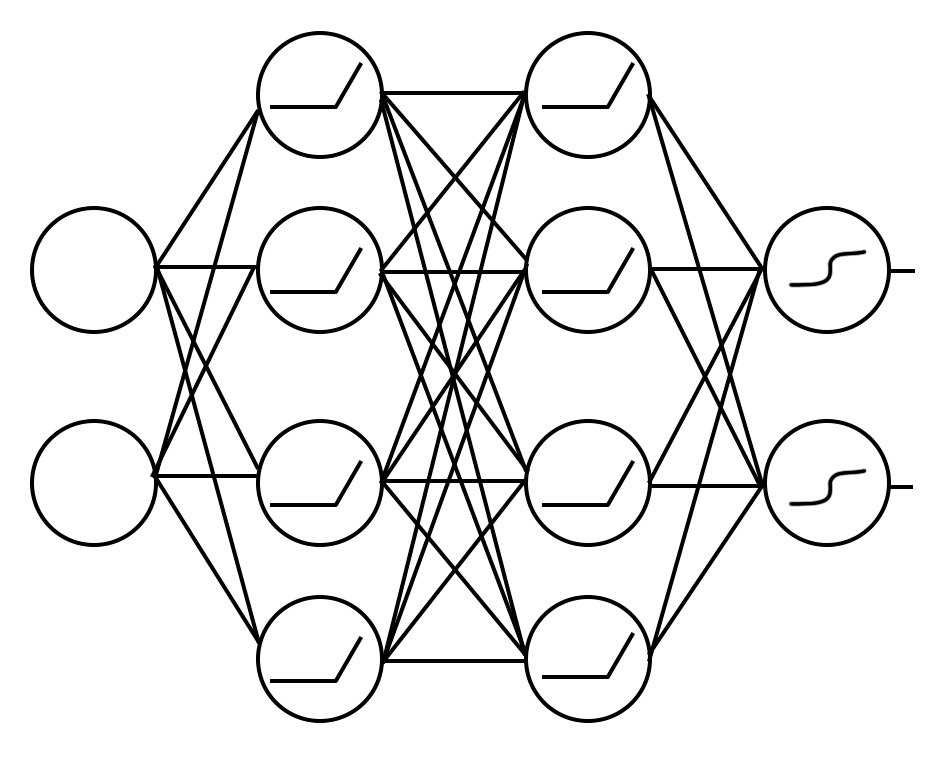
\includegraphics[width=75mm]{inst.png}
    \caption{Red neuronal del ejemplo de la instancia}
    \label{inst}
\end{figure}
Por ultimo se tiene un ultimo archivo que contiene la clase para las capas convolucionales, esta clase solo hace uso de la función de convolución definida anteriormente y hace el proceso de agrupar los resultados de aplicar todos los kernel:
\begin{lstlisting}[language=python]
class ConvNet():
def __init__(self,layers):
    self.layers = layers

def process(self,inputImage):
    original_image = inputImage.copy()
    neurons_results = []
    for j in self.layers:
        inputImage = original_image.copy()
        for i in j:
            if i[0] == "Convolution":
                inputImage = Convolutions.crossCorr2d(inputImage, i[1], padding=i[2])
            elif i[0] == "Pooling":
                inputImage = Pooling.max_pooling(inputImage,i[1],i[2])
            elif i[0] == "RELU":
                inputImage = RELU.RELU(inputImage)
        neurons_results.append(inputImage)
    return np.array(neurons_results)
\end{lstlisting}
\subsection{Arquitectura de la red neuronal del problema}
El resultado de experimentar con distintas arquitecturas es una red neuronal con una capa de convolución sin padding, con los kernerls diagonales, verticales y horizontales. 
El resultado de la capa de convolución es un vector de tamaño $1024\times1$ el cual es usado como entrada a la capa densa. Las capa densa esta formada por la capa de entradas que se dirige hacia la capa de salida, que da como resultado un
vector de tamaño $26\times1$, las posiciones de este vector representan cada una de las letras del abecedario en ingles. Esta ultima capa utiliza una función de activación sigmoidal, lo que regresa la probabilidad de que la entrada sea una de las 26 letras.
Se utiliza una tasa de aprendizaje de 0.5 y se entrena por 500,000 iteraciones. Los pesos y los sesgos son guardados en archivos de texto al instanciar la red y utilizados actualizados despues de ser entrenada. El código correspondinete a la inicialización de la red neuronal es le siguiente:
\begin{lstlisting}[language=python]
import numpy as np
import getData
import NeuralNetworks as NN
import sys
#Architecture
n = 1024
neurons = [n,26]
activation = ["sigmoid"]
error = "SE"
learning_rate = 0.3
NN1 = NN.NeuralNetwork(neurons, activation, error, learning_rate)
getData.storeData("weights.txt", NN1.weights,"w")
getData.storeData("biases.txt", NN1.biases,"w")
file = open("architecture.txt","w")
for i in range(len(neurons)):
    string = str(neurons[i])+","
    if i == len(neurons) - 1:
        string = str(neurons[i])
    file.write(string)
file.write("\n")
for i in range(len(activation)):
    string = activation[i]+","
    if i == len(activation) - 1:
        string = activation[i]
    file.write(string)
file.write("\n")
file.write(error+"\n")
file.write(str(learning_rate)+"\n")
file.close()
\end{lstlisting}
En el código se puede observar también los bloques correspondientes a la escritura de los pesos en archivos.
El archivo correspondiente al entrenamiento de la red neuronal es el siguiente:
\begin{lstlisting}[language=python]
import numpy as np 
import sys
import getData
import NeuralNetworks as NN
import ConvNet as CN
import Kernels

weights = getData.readData("weights.txt")
biases = getData.readData("biases.txt")
neurons, activation, error, learning_rate = getData.readArchitecture("architecture.txt")
NN1 = NN.NeuralNetwork(neurons, activation, error, learning_rate, weights=weights, biases=biases)
#Preparing input data
inputs = getData.readData("trainingData.txt")
targets = getData.readData("targetData.txt")
n = 18
newInputs = []
for i in range(len(inputs)):
    counter = 0
    newMatrix = []
    for j in range(n):
        newRows = []
        for k in range(n):
            newRows.append(inputs[i][counter].item())
            counter += 1
        newMatrix.append(newRows)
    newMatrix = np.asarray(newMatrix)
    newInputs.append(newMatrix)

# Intantiate Conv Layers
padding = False
ConvLayers = CN.ConvNet(
    [
        [["Convolution", Kernels.diagonal_left, padding] ],
        [["Convolution", Kernels.diagonal_right, padding]],
        [["Convolution", Kernels.vertical_line, padding]],
        [["Convolution", Kernels.horizontal_line, padding]]
    ]
    )     

iterations = 500000
print(len(inputs))
for i in range(iterations):
    actual_input = ConvLayers.process(newInputs[i % len(inputs)])
    actual_input = actual_input.flatten()
    actual_input = actual_input.reshape((len(actual_input),1))
    actual_target = targets[i % len(targets)]
    NN1.train(actual_input, actual_target)
    print("MSE:", np.power(NN1.error,2).sum()/len(NN1.error))
    print(i)
print("Trained")
getData.storeData("weights.txt", NN1.weights,"w")
getData.storeData("biases.txt", NN1.biases,"w")
\end{lstlisting}
Como se puede observar, este archivo implementa cada uno de los archivos anteriormente mencionados, el proceso de entrenamieneto se lleva acabo en un ciclo final 
que dura la cantidad de iteraciones asignada. Al terminar el entrenamiento los pesos y los sesgos se escriben directamente en los archivos
Una vez teniendo esto solo es cuestión de que la aplicación web envié una petición al servidor y ejecute el siguiente script de python:
\begin{lstlisting}[language=python]
import numpy as np 
import sys
import getData
import NeuralNetworks as NN
import ConvNet as CN
import Kernels
import string as st
try:
    #Preparing input data
    input_data = getData.parseRequestData(sys.argv[1], sys.argv[2], "c")
    # Intantiate Conv Layers
    padding = False
    ConvLayers = CN.ConvNet(
        [[["Convolution", Kernels.diagonal_left, padding] ],[["Convolution", Kernels.diagonal_right, padding]],
        [["Convolution", Kernels.vertical_line, padding]],[["Convolution", Kernels.horizontal_line, padding]]])     
    result = ConvLayers.process(input_data)
    result = result.flatten()
    result = result.reshape((len(result),1))
    #Intantiate Network from saved files
    weights = getData.readData("./backend/weights.txt")
    biases = getData.readData("./backend/biases.txt")
    neurons, activation, error, learning_rate = getData.readArchitecture("./backend/architecture.txt")
    NN1 = NN.NeuralNetwork(neurons, activation, error, learning_rate, weights=weights, biases=biases)
    print(st.ascii_lowercase[np.argmax(NN1.predict(result))])
except Exception as e:
    print("Final error:",e)
\end{lstlisting}
Una vez ejecutado el proceso de python el servidor recibe la respuesta de la red, y la envía al fronend de la aplicación donde muestra la letra que la red predijo.
\subsection{Conclusiones}
El proyecto se trabajó en parejas, por un lado la compañera Sonia Alejandra Treviño Rivera se encargó de la aplicación web, del preprocesamiento de datos entre el servidor y python y de la generación del conjunto 
de datos de entrnamiento de la red. Mientras que el compañero Edson Raul Cepeda Marquez se encargo de desarrollar el código correspondiente a la red neuronal y los algoritmos correspondientes. Los problemas principales eran muy variados,
desde fallás en la lógica de la programación de los algoritmos, hasta problemas de comunicación entre la aplicación y el servidor. Estos problemas fueron resueltos en equipo recibiendo retroalimentación de cada uno e ideas para la resolución de estos problemas. 
Una de las cosas que se puede compartir de esto, es que desarrollar los algoritmos de aprendizage automatico desde cero no es lo lo más eficiente, pero en cuestiones didacticas deja unas buenas bases del tema, lo que despues se traduce en la facilidad para usar
librerias. Todo lo expuesto a lo largo del documento fue comprendido en su totalidad, por lo que los conocimientos adquiridos se ven reflejados en este documento. 
Debido a la falta de tiempo, el conjunto de datos no es lo que esperabamos, se planeaba por lo menos 100 ejemplos por cada letra para que la red neuronal fuera entrenada de manera correcta, pero conseguimos hacer 30 por cada letra. Lo que de todos modos
resulto en un porcentaje de exito del 80\% de las predicciones de la red.
\begin{thebibliography}{9}

    \bibitem{NND} 
    Hagan, M. (2014). Neural Network Design. Ok, Estados Unidos.
    \bibitem{Linear} 
    Poole, D. (2015) Linear Algebra: A modern introduction. Stamford, CT. 
    \bibitem{conv} 
    Pokharna, H. (2016, 28 de julio). The best explanation of Convolutional Neural Networks. \\
    Recuperado de: \texttt{https://medium.com/technologymadeeasy} \\
    \texttt{/the-best-explanation-of-convolutional-neural-networks-on-the-internet-fbb8b1ad5df8}
    
    \bibitem{sharm} 
    Sharma, S. (2017, 6 de septiembre). Activation Functions in Neural Networks \\
    Recuperado de: \texttt{https://setosa.io/ev/image-kernels/}
    
    
    \bibitem{powell} 
    Powell, V. (2018). Image Kernels explained Visually
     \\
    Recuperado de: \texttt{https://towardsdatascience.com/activation-functions-neural-networks-1cbd9f8d91d6}
    
    
    \bibitem{codigo1}
    Edson Cepeda, Neural Networks, Github repository: \\
    \texttt{https://github.com/OrbitalCardinal/NeuralNetworks}
    
    \end{thebibliography}
\end{document}
